\documentclass[12pt,a4paper]{article}
\usepackage[utf8]{inputenc}
\usepackage[T1]{fontenc}
\usepackage[provide=*,french]{babel}
\usepackage{graphicx}
\usepackage{geometry}

\geometry{margin=2.5cm}

\begin{document}

% Page de garde
\begin{titlepage}
    \begin{center}
        \vspace*{2cm}
        {\huge\bfseries Devoir 3\par}
        {INFO4305\par}
        \vspace{2cm}
        {\Large Alec Jones\par}
        {\large A00216262\par}
        \vfill
    \end{center}
\end{titlepage}

\tableofcontents
\newpage

% Introduction
\section{Introduction}

% Objectif
\section{Objectif du TP}
 [Les objectifs du TP]

% Corps du rapport
\section{Déroulement du TP}
\subsection{Partie 1}
Premièrement on doit d'abord installer Gpg4win, j'ai installer le logiciel à
l'aide du manager de paquets WinGet.

\begin{figure}[h]
    \centering
    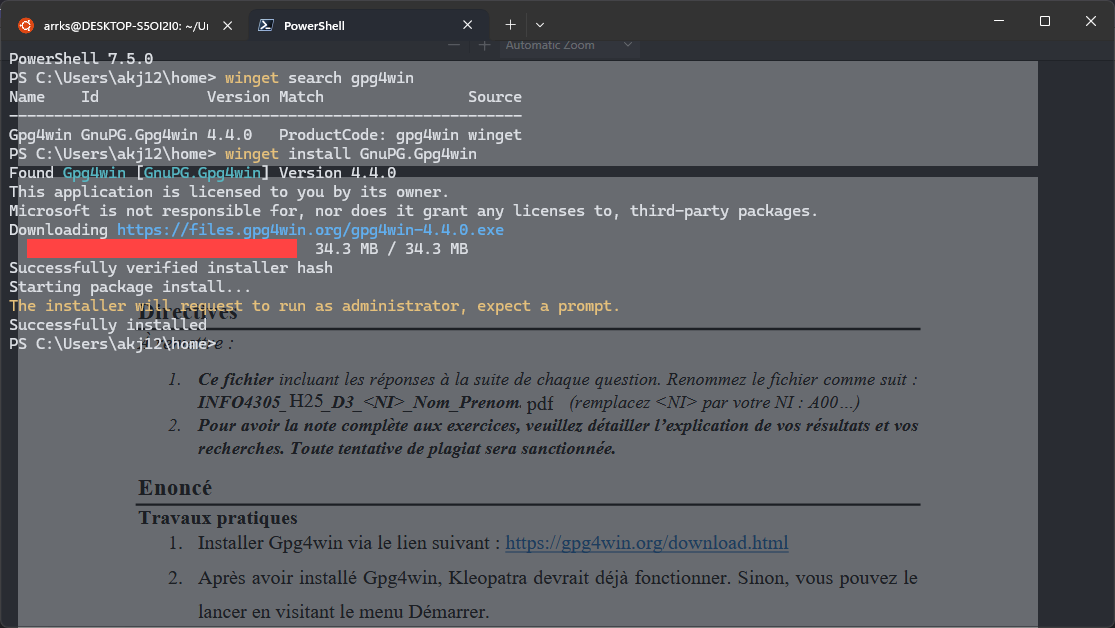
\includegraphics[width=0.8\textwidth]{../img/image.png}
    \caption{Installation de Gpg4win}
\end{figure}

\subsection{Partie 2}


% Conclusion
\section{Observation, interprétation et conclusion}
 [Vos observations et conclusions]
\begin{itemize}
    \item Objectifs atteints ou non
    \item Ce que vous avez accompli
    \item Ce que vous avez compris
\end{itemize}

\end{document}
